\documentclass[margin,line]{res}
\usepackage{graphicx}
\usepackage{hyperref}
\usepackage{url}
\oddsidemargin -.5in
\evensidemargin -.5in
\textwidth=6.0in
\itemsep=0in
\parsep=0in
\topmargin=0in
\topskip=0in
 
\newenvironment{list1}{
  \begin{list}{\ding{113}}{%
      \setlength{\itemsep}{0in}
      \setlength{\parsep}{0in} \setlength{\parskip}{0in}
      \setlength{\topsep}{0in} \setlength{\partopsep}{0in}
      \setlength{\leftmargin}{0.17in}}}{\end{list}}
\newenvironment{list2}{
  \begin{list}{$\bullet$}{%
      \setlength{\itemsep}{0in}
      \setlength{\parsep}{0in} \setlength{\parskip}{0in}
      \setlength{\topsep}{0in} \setlength{\partopsep}{0in}
      \setlength{\leftmargin}{0.2in}}}{\end{list}}


    
\begin{document}
\name{\LARGE N.MUTHU KARUPPAN} \hfill {\em \today}

\begin{resume}
\section{\sc CONTACT INFORMATION}

\vspace{.05in}
\begin{tabular}{@{}p{3.5in}p{3in}}
D246, Anna Nagar,           & {Phone:}  09047057904 \\
1st Cross, Tennur, Trichy-620017
 & {E-mail:}  muthukaruppannachiappan@gmail.com\\
\end{tabular}

\section{\sc Photo}
\begin{figure}[hbt]
  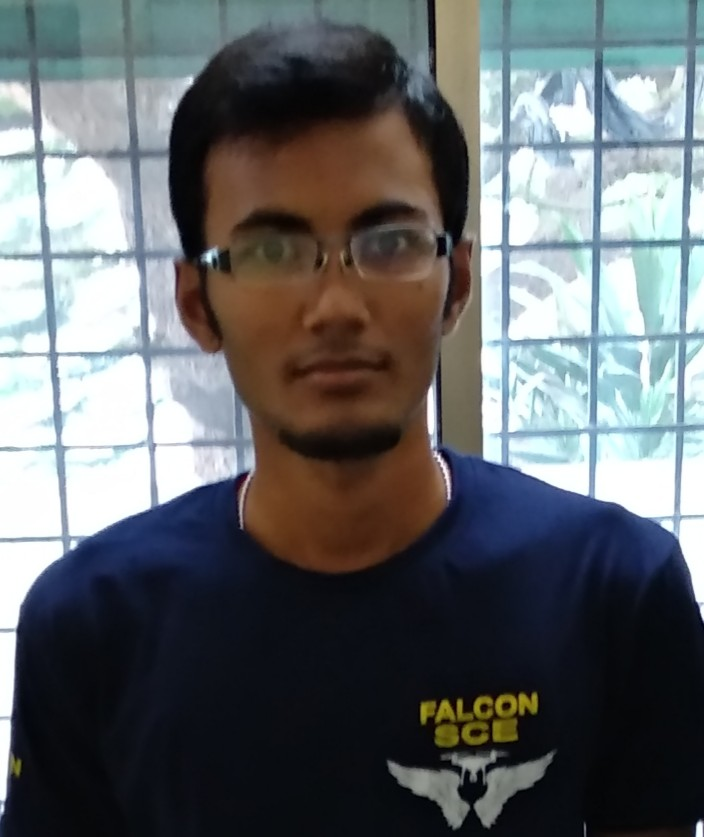
\includegraphics[width=5cm,height=5cm,keepaspectratio, angle= 0]{muthu.jpg}
\end{figure}


\section{\sc OBJECTIVE}

Seeking a postion to utilize my Skills and Abilites in the organisation as an Engineer that offers Professional Growth and Opportunities to Explore new concepts while being Resourceful, Innovative and Adaptable.\\

\section{\sc OBJECTIVE EDUCATION:}
\begin{tabular}{|c|c|c|c|c|}
\hline
&&&&\\
\textbf{Degree}	&	\textbf{Institution}	&	\textbf{University/Board}	&	\textbf{Passing Year}	&	\textbf{Pass Percentage}\\
&&&&\\ \hline

&&&&\\
B.E &Saranathan&Anna &2019&7.33\\ 
(Electrical&College of&University& &(upto 5th\\
and Electronics)&Engineering& & &semester)\\ 
&&&&\\ \hline

&&&&\\
HSC&Sri Jayendra&State board&2015&82.75\\
 &Matriculation&Board&&\\
 &Higher Secondary School&&&\\ 
&&&&\\ \hline

&&&&\\
 SSLC&Mahatma Gandhi&CBSE&2013&94\\
 &Centenary Vidhyalaya&&&\\ 
 &&&&\\ \hline
\end{tabular}


\section{\sc PROJECTS}
%%%%%%
{\em Main Project}\\
\begin{enumerate}
\item \textbf{Title:} APCTMD (Air Pollution Control and Traffic Management Drone) for Smart City Development in eYIC-2018(e-Yantra Ideas Competition)[Team Representative].\\
\item \textbf{Title:} Sharik in NSVC (National Solar Vehicle Challenge).\\
\end{enumerate}

{\em Mini Project}\\
\begin{enumerate}
\item \textbf{Title:} Voice Controlled Robot using Arduino [Team Representative].\\
\item \textbf{Title:} Swarm Robots using Arduino [Team Representative].\\
\item \textbf{Title:} ECO-HOOP (App controlled Wheel chair).\\
\item \textbf{Title:} Line Follower Robot using Arduino [Team Representative].\\
\end{enumerate}
%%%%%%%%%%%


\section{\sc TRAININGS UNDERGONE}
\begin{itemize}
\item In-plant Training in Central Workshops, Golden Rock, Southern Railways, Ponmalai-620 004 during the period from 19th June 2017 to 24th June 2017.\\
\item AutoCAD, ECAD, ORCAD courses certified By IASC (Instrumentation Automation Surveillance and Communication Sector Council) and partnered with Skill India and NSDC (National Skill Development Council).\\
\end{itemize}
%%%%%%

\section{\sc TECHNICAL SKILLS}
\begin{enumerate}
\item Simulation in ORCAD, ECAD and MATLAB.\\
\item Fabrication of electronic circuits in PCB board in PROTEUS.\\
\item Modelling in AutoCAD Classic.\\
\item Familiar with CCS (Code Composer Studio) and Energia.\\
\end{enumerate}

\section{\sc SOFTWARE SKILLS}
\begin{enumerate}
\item \textbf{Operating System:} Windows XP, 7, 8 and 10.
\item \textbf{Language:} Basic C, C++, Embedded C, Python and java.
\item  \textbf{Others:} MS-Word, MS-Excel, MS-PowerPoint.
\end{enumerate}

\section{\sc AREA OF INTEREST}
\begin{itemize}
\item Robotics
\item Quadcopter
\end{itemize}


\section{\sc SOFT SKILLS}
\begin{itemize}
\item Leadership
\item Ability to work in a team
\item A better analyzer
\item Optimistic
\item Smart solution finder
\end{itemize}

\section{\sc PROFESSIONAL BODIES MEMBERSHIP}
\begin{enumerate}
\item Institution Of Engineers (IEI)
\item Society of Automotive Engineers (SAE)
\end{enumerate}

\section{\sc COMPETITIONS PARTICIPATED}
\begin{itemize}
\item One of the 18 Finalist teams out of 318 teams in eYIC-2018(e-Yantra Ideas Competition) event conducted by IIT-Bombay Sponsored by MHRD (Ministry of Human Resource Development), Government of India, under the NMEICT (National Mission on Education through Information and Communication Technology).
\item Participated in NSVC 2017-18 (National Solar Vehicle Challenge) and secured 14th place out of 37 teams.
\item Participated in NSVC 2017-18 (National Solar Vehicle Challenge) and ranked National level 4th in Virtual Round.
\item Participated in PRATIG Project Expo 2018 conducted by Saranathan College of Engineering and successfully completed the Multi-Disciplinary Project Title ECO-HOOP (App Controlled Wheel Chair).
\item Participated in Mini Project contest conducted by Energy Club of Saranathan College of Engineering and Won the 1st prize in the contest.
\item Participated in Mini Project contest conducted by Saranathan College of Engineering and Won the 1st prize in the contest.
\item Participated in APPMANIA 2017 contest conducted Saranathan College of Engineering and created a Relay Go Android App under 12hrs in the contest.
\end{itemize}

\section{\sc WORKSHOPS ATTENDED}
\begin{enumerate}
\item Participated in “QUADCOPTER” workshop organized by PRAGYAN ’17, the International Techno – Managerial Organization of NIT Tiruchirappalli, Trichy held from 2nd March 2017 to 5th March 2017.
\item Participated in “C2000 REAL-TIME CONTROLLER” workshop organized by PRAGYAN ’18, NIT Tiruchirappalli, Trichy held from 3rd March 2018 to 4th March 2018.
\item Participated in “SMART SORTER ROBOTIC ARM” workshop organized by SENSORS ’18, the National Level Technical Symposium of Department of ICE, NIT Tiruchirappalli, Trichy held from 29th January 2018 to 30th January 2018.
\item Participated in “FUNCTION GENERATOR USING OP-AMP” workshop organized by Research cell-EEE, Saranathan College of Engineering, Trichy held on 9th January 2017.
\item Participated in “INTERNATIONAL WORKSHOP ON ARDUINO IN ROBOTICS” workshop organized by LansA Informatics Pvt Ltd and Thick India held on 18th December 2016 at Coimbatore Institute of Technology.
\item Participated in “EMBEDDED AND ROBOTICS” workshop organized by iSYSWAYS Technologies held on 21st August 2016 at Tanjore.
\end{enumerate}

\section{\sc CERTIFICATIONS}
\begin{itemize}
\item Certificate for Completion of C Training offered by the Spoken Tutorial Project, IIT Bombay, funded by National Mission on Education through ICT, MHRD, Govt ., of India .
\item Certificate for Completion of C++ Training offered by the Spoken Tutorial Project, IIT Bombay, funded by National Mission on Education through ICT, MHRD, Govt ., of India .
\item Certificate for Completion of JAVA Training offered by the Spoken Tutorial Project, IIT Bombay, funded by National Mission on Education through ICT, MHRD, Govt ., of India .
\item Certificate for Employability Skill Test offered by Wheebox and successfully secured India wide 76th Rercentile Rank.
\item Attended Orientation Program in Entrepreneurship (WFNEN-100) conducted by WADHWANI Foundation and National Entrepreneurship Network in Learnwise. 
\end{itemize}

\section{\sc OTHER CREDENTIALS}
\begin{enumerate}
\item Participated in Chess Rating tournament conducted by AICF.
\item Won State level and district level prizes in chess tournaments.
\item Zonal Winners in Chess Tournament 2015 and 2016 conducted by Anna University.
\item Chess Tournament Runners in Inter-Department sports 2016, 2017 and  2018 conducted by Saranathan College of Engineering.
\item Zonal Runners in Kho-Kho tournament.
\end{enumerate}

\section{\sc RELAXATION AND INTEREST}
\begin{itemize}
\item Reading Books.
\item Playing Chess and Carrom.
\item Pencil sketching and craft works.
\item Solving Rubix cube.
\end{itemize}


\section{\sc PERSONAL DETAILS}
\begin{itemize}
\item \textbf{Father’s Name:} Mr. RM. Nachiappan
\item \textbf{Mother’s Name:} Mrs. N. Meenakshi
\item \textbf{Date of Birth:} 14-02-1998
\item \textbf{Gender:} Male
\item \textbf{Nationlity:} Indian
\item \textbf{Maruital Status:}Single
\item \textbf{Languages Known:} Tamil, English
\end{itemize}

\section{\sc REFERENCEs}
\begin{itemize}
\item \textbf{Dr. D.Vallavan} Principal, Saranathan College of Engineering, Trichy\\
\textbf{Email:}principal@saranathan.ac.in\\
\item \textbf{Dr. C.Krishnakumar} Head of the Department / Electrical and Electronics Engineering, Saranathan College of Engineering, Trichy\\
\textbf{Email:}krishnakumar-eee@saranathan.ac.in\\
\item \textbf{Ms. N.Gayathri} Assistant Professor, Department of  Electrical and Electronics Engineering, Saranathan College of Engineering, Trichy\\
\textbf{Email:}gayathri-eee@saranathan.ac.in\\
\end{itemize}

\section{\sc DECLARATION}
I declare that the information furnished above is true and correct to the best of my knowledge and belief.\\

\section{\sc DATE}
19 April 2018\\

\end{resume}
\end{document}




